\section{Semaine 02 (23/09-27/09) }


\e{Notions abordées :}
\begin{itemize}
	\item Circuits linéaires du premier ordre.
\end{itemize}

\subsection{Questions de cours}
\begin{enumerate}
	\item Relation entre la charge d'un condensateur et sa tension aux bornes.
	\item Relations entre intensité et tension pour un condensateur et une bobine.
	\item Continuité des grandeurs dans un circuit électrique.
	\item Établir l'expression de l'énergie stockée dans un condensateur/une bobine.
\end{enumerate}

\subsection{Exercice 1 : Résistance de fuite d'un condensateur}

Un condensateur réel présente des fuites de courants. Comment le modéliser ?

Il est inséré dans un circuit série comportant un générateur de f.é.m $E$, une résistance $r$ et un interrupteur $K$. On mesure la tension aux bornes du condensateur à l'aide d'un voltmètre idéal. On ferme $K$ et on attend que l'indication du voltmètre se stabilise. Puis on ouvre K en déclenchant au même instant un chronomètre. On constate que la tension indiquée par le voltmètre baisse de $10\%$ en un temps $T$.

On donne $E = \SI{1}{V}$, $r=\SI{10}{k\Omega}$, $T=\SI{1.0}{s}$ et $C=\SI{19}{\mu F}$.

\begin{enumerate}
	\item Exprimer la valeur $U$ vers laquelle la tension aux bornes du condensateur tend lorsque $K$ est fermé. En déduire une manière de déterminer $R_f$ (résistance de fuite).
	\item Montrer que la mesure du temps $T$ permet aussi de déterminer $R_f$. Commenter en relation avec l'une des hypothèses de l'énoncé.
\end{enumerate}

\subsection{Exercice 2 : Étude d'un circuit RL}

\begin{minipage}[c]{\linewidth/2}
	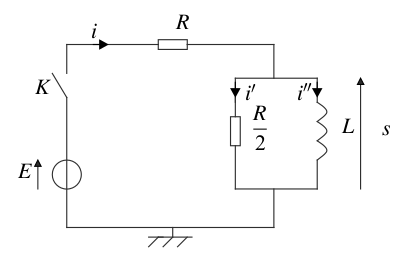
\includegraphics[width=\linewidth]{Images/mpsi_s02_ex02.png}
\end{minipage}%
\begin{minipage}[c]{\linewidth/2}
	À $t=0^-$, on ferme l'interrupteur $K$.
	\begin{enumerate}
		\item Donner $i$, $i'$, $i''$ et $s$ en $t=0^+$.
		\item Que vaut $s(t)$ lorsque $t$ tend vers l'infini.
		\item Établir l'équation différentielle vérifiée par $s(t)$.
		\item En déduire $s(t)$. En tracer l'allure.
		\item Exprimer le temps $t_0$ au bout duquel $s(t)$ a été divisé par $10$.
		\item On mesure $t_0=\SI{30}{\mu s}$ pour $R=\SI{1.0}{k\Omega}$. En déduire $L$.
	\end{enumerate}
\end{minipage}

\subsection{Exercice 3 : Rendement énergétique de la charge d'un condensateur}

On considère un circuit composé d'une résistance $R$ et d'un condensateur de capacité $C$ en série aux bornes duquel on place un générateur de tension idéal de f.é.m $E$ et un interrupteur $K$. À l'instant $t=0$, on ferme l'interrupteur $K$ et la tension $u_c$ aux bornes du condensateur est nulle.

\begin{enumerate}
	\item Établir l'équation différentielle vérifiée par $u_c$.
	\item Déterminer $u_c(t)$ et en tracer l'allure.
	\item Mêmes questions pour l'intensité du courant parcourant le circuit.
	\item Exprimer en fonction de $C$ et $E$ :
	\begin{itemize}
		\item L'énergie $\mathcal{E}_{elec}$ emmagasinée par le condensateur quand $t\rightarrow+\infty$.
		\item L'énergie $W_{Joule}$ dissipée par effet Joule dans la résistance entre $t=0$ et $t\rightarrow+\infty$.
		\item L'énergie $W_{gen}$ fournie par le générateur entre $t=0$ et $t\rightarrow+\infty$.
	\end{itemize}
	\item Donner une relation liant $\mathcal{E}_{elec}$, $W_{Joule}$ et $W_{gen}$ et proposer une interprétation physique de cette relation. Comment définir puis exprimer un rendement ?

\end{enumerate}